\documentclass[11pt, twocolumn]{article}
\usepackage[scale=.87]{geometry}
\usepackage{hyperref}
\usepackage{cite} % BiTeX
\usepackage[square]{natbib}
\usepackage{amsmath}
\usepackage{graphicx}
\newcommand{\ts}{\textsuperscript}
\newcommand{\HRule}{\rule{\linewidth}{0.5mm}}

\begin{document}

\twocolumn[\begin{@twocolumnfalse}
\begin{center}
    \begin{large}
    {\HRule \\[0.2cm]}
    \textsc{\Huge SMARTer 2020 review}
    {\HRule \\[0.3cm]}
    \end{large}

    \begin{minipage}{ 0.49\textwidth }
        \begin{flushleft}
            Kacper \textbf{Sokol}---\texttt{ks1591}---4GGK1\\
            \today
        \end{flushleft}
    \end{minipage}
    \begin{minipage}{ 0.49\textwidth }
        \begin{flushright}
            {Sustainability, Technology and Business\\
             COMSM0006; University of Bristol, UK\\[0.3cm]}
        \end{flushright}
    \end{minipage}
\end{center}
\vspace*{1em}\end{@twocolumnfalse}]

{\small\noindent Glossary
\begin{description}
\item[BAU] Business as Usual
\item[$\mathbf{CO_2e}$] $CO_2$ equivalents
\item[GHG] Green House Gases
\item[ICT] Information Communications Technology
\item[PV] photo voltaic
\item[T\&D] Transmission and Distribution
\item[the report/paper] SMARTer 2020 report
\item[VPP] Virtual Power Plant
\end{description}}

\section{Introduction}
World's economy is developing in incredible pace, improving our everyday life. Despite all the advancements in technology, especially in ICT, the \emph{global warming} problem mainly caused by GHG (with major contribution of $CO_2$) emitted by burning fossil fuels, has not been paid enough attention to ensure sustainable development. It should be our goal to reduce GHG emission and decouple its increasing production from economic growth to keep the environment clean and in best shape for future generations.\\

ICT enabled technologies can be used to reduce emission from sectors like: power generation, transportation, manufacturing, service \& consumer, agriculture \& land use, and buildings. The main advantage of such solutions is relatively low emission footprint from incorporating the technology in comparison to possible abatement potential it enables yielding overall positive emission balance.\\
Implicit advantages of these technologies are additional job openings and significant long or short term financial savings.\\

Estimating potential $CO_2\mathbf{e}$ saving with high accuracy is challenging task due to many overlays in addressed sublevers, different economic and political potential of countries, and constantly emerging technologies giving rise to new abatement potential.\\

This review focuses on \emph{Power} end-use sector as it necessary factor for all other sectors and it contributes major part of proposed in \citep{global2012smarter} reduction scheme.

\section{Power sector overview}
The \emph{Power} end-use sector can be divided as shown in \emph{table}~\ref{tab:powersublevers}. Its overall addressable emission is the highest out of all sectors proposed in the report and sums up to: $\mathbf{2.02} \mathbf{Gt}CO_2\mathbf{e}$. Four countries constituting for almost half of this abatement are: \emph{China}, \emph{United States}, \emph{Germany}, and \emph{India}; with respective contribution of: $\mathbf{0.390} \mathbf{Gt}CO_2\mathbf{e}$, $\mathbf{0.350} \mathbf{Gt}CO_2\mathbf{e}$, $\mathbf{0.040} \mathbf{Gt}CO_2\mathbf{e}$, and $\mathbf{0.143} \mathbf{Gt}CO_2\mathbf{e}$ with total of $\mathbf{0.923} \mathbf{Gt}CO_2\mathbf{e}$.

\begin{center}
  \begin{table}[h]
    \begin{tabular}{ p{.225\textwidth} | p{.225\textwidth} }%{ p{10.5em} | p{10.5em} }
      Integration of renewables & Smart grid enabling \\
      \hline
      Demand management;\newline Time-of-day pricing;\newline Power-load balancing;\newline Power grid optimization & Integration of renewables in power generation;\newline Virtual power plant;\newline Integration of off-grid renewables and storage
    \end{tabular}
    \caption{Sublevers in \emph{Power} sector.\label{tab:powersublevers}}
  \end{table}
\end{center}

Each sublever addresses different part of power sector:
\begin{description}
\item[Demand management] is a mechanism to manage electricity consumption in response to supply conditions; it is reducing non-base load electricity.

\item[Time-of-day pricing] is variable electricity pricing mechanism for different times of day; it allows customer to adjust their consumption and reduce overall demand on the grid during peak hours; it is reducing non-base load electricity.

\item[Power-load balancing] are various techniques to store overhead of produced electricity during low demand and release it during peak hours to support generation; it is reducing non-base load electricity.

\item[Power grid optimization] reduces inefficiencies of energy transmission \& distribution and optimises infrastructure with use of ICT---gathering and acting upon information e.g.\ detecting and prosecuting power theft; it is reducing emission of power generation.

\item[Integration of renewables in power generation] integrates the off-grid renewables and ensures more efficient use of them with use of ICT---e.g.\ by storing the overhead; it is reducing emission of power generation.

\item[Virtual power plant] are collectively run distributed generation installations managed by ICT infrastructure---e.g.\ in the neighbourhood; it is reducing emission of power generation.

\item[Integration of off-grid renewables and storage] integrates storage into off-grid power loads with use of ICT; it is reducing emission form off-grid fossil fuel power generators.
\end{description}

And, each country has distinctive background with different problems to overcome:
\subsection{China}
China's economy is one of the most powerful in the world and uses high amount of electricity nevertheless, low energy prices prevent uptake of any upgrade to power infrastructure. The grid infrastructure needs an update to facilitate rapid development of presented below ICT enabled solution hence, \emph{power grid optimisation} has the greatest abatement potential.\\
Unfortunately, at the moment government has monopoly on power market yielding no competition driving the development of the power infrastructure. It has been well known issue for some time now, but the situation has not changed hence presented in \emph{the report} plans may partially fail as competition driven improvements are assumed.\\
Moreover, government movement to secure high peak demand with relatively dirty ``peak power plants'' (which otherwise stay idle) rather than trying to shift the demand indicates low involvement in reduction plans. To introduce changes in China's \emph{power} sector government intervention is needed as majority of proposed in \emph{the report} improvements lacks strong business case due to long return time, and high upfront costs with no subsidiaries or special loans.\\

\subsection{United States}
The United States is well developed country with high usage of energy produced by dirty energy mix (37\% coal) and delivered by old and inefficient grid; the power sector contributes 42\% to US emissions. Fortunately, over the last decade energy generation emission decreased as US is shifting from coal to cleaner sources like natural gas.\\
Major part (82\%) of the power abatement potential in the US is due to \emph{integration of renewables in power generation} and \emph{power grid optimisation}. It may be hard to introduce changes proposed in these sublevers as US domestic oil and gas resources as well as low energy taxes cause low energy prices yielding low interest in renewable energy and grid upgrades.\\
Due to this reasons business case for majority of sublevers is weak hence government intervention and subsidiaries are needed to boost the market. Unfortunately, at the moment there are little general, country-wide laws encouraging to use renewables like state specific \emph{investment tax credit} and \emph{production tax credit}. Majority of the decision is left up to particular state however \emph{net metering policy} is used country-wide so energy overproduced by customers can be sold back to the grid for the retail price---which is fairly low leading to low interest.\\
To boost the uptake of ICT in power sector country-wide government incentives are needed as ICT-enabled technologies have high introductory costs and low repay rate. Investment in research is also essential to reduce costs of technologies in long term, and to address near future government direct incentives like subsidies and rebates for investments in ICT, and stronger \emph{renewable portfolio standards} is needed. To achieve greatest potential full deployment has to be done in one run: \emph{time of day pricing} and \emph{demand management} depend on implementation of smart meters---without covering whole technology suit they are simply ineffective. Therefore, to achieve the proposed abatement potential electricity price market regulations (e.g.\ dynamic pricing or pricing for carbon), incentives, and penalties are needed to boost the innovations.\\

\subsection{Germany}
Since 1990 German's emission is steadily declining despite little improvements over the years and continuous dependence of power sector on fossil fuels.\\
Germany set clear and ambitious GHG abatement roadmap for upcoming decade---\emph{Energiewende} (energy transformation) plan was introduced to reduce GHG emission in energy generation by installing renewable energy sources. The plan aims at producing 35\% of energy from renewable sources by 2020, and 80\% by 2050. These assumptions seems viable as in first half of 2012 the share of renewable energy in power generation exceeded 25\% nevertheless, the first step towards this goal is developing each sublever that plays significant role in globally working system.\\
The obstacle that may delay German government in realising these plans is country's decision to phase out relatively clean nuclear power plants currently constituting 22\% of power mix. To avoid increase in emission it must be replaced with renewable energy which on the other hand will not significantly reduce overall GHG emission as fossil-fuel generation will remain intact.\\

\subsection{India}
India is developing country with continuously improving people's wealth, leading to increase in demand for electrical power caused by appliances like TVs or air conditioners. GHG emission is still strongly linked with economic growth therefore it is projected to increase over next years.\\
Power sector is largest contributor to country's emission blamed on inefficient power grid, and high fossil fuel dependence (coal, natural gas, and oil). Electricity thefts which are not pursued are very common---especially in rural areas---and T\&D losses are estimated to be on average 22\%, reaching 50\% in some places. Furthermore limited grid connectivity causes many phone towers to run on dirty diesel generators. To improve this situation in 2011 TRAI mandated 50\% of rural and 20\% of urban towers to run on hybrid power by 2015, and 75\% urban and 33\% rural towers by 2020.\\
To improve poor energy infrastructure in 2008 Indian government introduced \emph{The National Action Plan on Climate Change} aiming at significantly reducing the emissions by 2017, reducing 2005 GHG emission by 20-25\% by 2020, and saving $10000 MW/year$ with appliance modernisation. One component of the plan is \emph{National Solar Mission} with goal of producing $1000 MW/year$ PV power, increasing overall wind capacity, and increasing renewable energy share 1\% per year to reach 15\% by 2020; with current penetration of about 2\%.\\
The major barrier for ICT enabled power sector is poor grid infrastructure hence major investments should be done in \emph{power grid optimisation} and \emph{integration of renewables} to prepare for modernisation. Currently the power network is not standardised and fractured with 78 different utilities making it difficult to integrate and enforce ICT improvements therefore ICT-enabled power infrastructure is unlikely to be built by 2020. \emph{The report} is not clear whether this risk is quantified in calculated abatement potential.\\
The main curdle for the abatement plan to be realised is lacking ICT-enabled smart grid required for majority of presented possibilities. The single sublever yielding instant shift of peak-demand is time-of-day pricing, which does not require advanced technologies for functioning. Recent work of ministry of power introduced \emph{Restructured Accelerated Power Development and Reforms Program (R-APDRP)} to promote smart meter deployment but low internet connectivity (7.5\% of Indians regularly use internet), and the lack of ICT abatement awareness prevents the spread of technology. Furthermore, currently 75\% of energy is produced by state distributors with government not paying for its electricity usage and sector having return rate of -18\% making weak business case for majority of presented sublevers.\\
Finally, presented case study shows grid-lacking villages powered by green powered smart grids giving cheap access to clean electricity, but producing energy from PV can be as high as 20 times more expensive than from coal making required infrastructure relatively expensive.


\section{Abatement potential and sublevers reconstruction}

\subsection{Demand management}
\subsubsection{Abatement potential review}
The report estimates power capacity of the world at $6.9 TW$ (not referenced) but it does not specify when this capacity was reached or will be reached. Moreover the assumption of $\mathbf{0.55} \mathbf{kg}CO_2\mathbf{e} / kWh$ emission rate is also not referenced. The saving ratio of $65 Wh/W$ (demand response) used in the report can be easily found in~\citep{grid2008green}. However, the referred paper notifies that data were collected for commercial buildings only and for the purpose of approximation they are used for residential buildings. Finally, saving potential of 4\% is estimated based on ``penetration from case studies'' and is referenced to~\citep{grid2008green} which does not contain such figure. It can be easily spotted that references in the table are mixed.\\
The emission rate used in the report to calculate abatement potential may be misleading, as due to power generation improvements over the years the emission factor should decrease causing lower overall abatement potential. Also some businesses may not be able to shave their energy use due to business characteristics leading to smaller overall abatement potential.\\

In China \emph{demand management} can save $\mathbf{4} \mathbf{Mt}CO_2\mathbf{e}$ according to text and $\mathbf{4.2} \mathbf{Mt}CO_2\mathbf{e}$ according to the corresponding table. This sublever is highly dependant on government actions such as issuing specific law as government involvement in power sector is significant. The aim in China is to reduce peak-load electricity which is also addressed in other sublevers leading to potential overlay with \emph{time-of-day pricing} and \emph{power load balancing}.\\
The report assumes country specific power capacity of $2 TW$ in 2020 and emission factor of $\mathbf{0.8} \mathbf{kg}CO_2\mathbf{e} / kWh$ both referenced ambiguously to \emph{IEA} leading to both figures being untraceable. The energy saving ratio and saving potential are the same as in worldwide calculations what may lead to inaccurate calculations as each country has different economic.\\

In the US this sublever can save $\mathbf{21} \mathbf{Mt}CO_2\mathbf{e}$ according to text and $\mathbf{1.4} \mathbf{Mt}CO_2\mathbf{e}$ according to the corresponding table what is an obvious mistake. This sublever targets at reducing peak-load electricity usage with help of: smart meters, smart-grid infrastructure, and changing customer behaviour. The first two indicate high dependence on smart-grid infrastructure which may not be ready at time and creates potential overlay. The last one might be difficult to achieve as it is dependent on behaviour of many people hence the assumption is risky.\\
The report assumes country specific power capacity of $1 TW$ in 2020 and emission factor of $\mathbf{0.55} \mathbf{kg}CO_2\mathbf{e} / kWh$ both referenced ambiguously to \emph{EIA} leading to both figures being untraceable. The energy saving ratio and saving potential are the same as in worldwide calculations what may lead to inaccurate calculations as each country has different economic.\\

In Germany this sublever can save $\mathbf{0.3} \mathbf{Mt}CO_2\mathbf{e}$ according to text and $\mathbf{1.4} \mathbf{Mt}CO_2\mathbf{e}$ according to the corresponding table what is an obvious mistake. Furthermore, it is clear that the sub-model details in this row are copy-and-paste error, and are taken from the US table as it says ``...capacity in US in 2020...''. The authors of the report claim small potential of this sublever on the country level but do not elaborate on it.\\

In India this sublever can save $\mathbf{1} \mathbf{Mt}CO_2\mathbf{e}$ according to text and $\mathbf{0.8} \mathbf{Mt}CO_2\mathbf{e}$ according to the corresponding table. It is inconsistently called here \emph{demand response} and it aims at reducing peak-load electricity, unfortunately India is lacking infrastructure for this sector to play significant role.\\
The report assumes country specific power capacity of $0.39 TW$ in 2020 and emission factor of $\mathbf{0.8} \mathbf{kg}CO_2\mathbf{e} / kWh$ both referenced ambiguously to~\citep{grid2008green} which does not contain both figures causing them to be untraceable. The energy saving ratio and saving potential are the same as in worldwide calculations what may lead to inaccurate calculations as each country has different economic.\\


\subsubsection{Sublever reconstruction\label{sec:dm:reconstruction}}
According to~\citep{eia2011} the world power capacity was $5.331045 TW$ in 2011, and the closest estimate that I could find for 2020 is $5.8 TW$ read from the graph in~\citep{2002:iba}. The capacities of: China, US, Germany, and India in 2011 are in order: $1.1 TW$, $1.1 TW$, $0.2 TW$, and $0.2 TW$ (\citep{eia2011}). The estimations for 2020 could not be found.\\
The average world emission rate according to~\citep{iea2012co2} is $\mathbf{0.534 kg}CO_2\mathbf{e}/\mathbf{kWh}$ and country specific figures are (order preserved): $\mathbf{0.790 kg}CO_2\mathbf{e}/\mathbf{kWh}$, $\mathbf{0.528 kg}CO_2\mathbf{e}/\mathbf{kWh}$, $\mathbf{0.468 kg}CO_2\mathbf{e}/\mathbf{kWh}$, and $\mathbf{0.936 kg}CO_2\mathbf{e}/\mathbf{kWh}$.\\
Finally, the report states 4\% saving potential referring to~\citep{grid2008green}, but the source estimates saving potential as 5\% with strong assumption of 43\% of customers implementing a cost-effective combination of demand response enabling technologies. Applying 5\% value instead of 4\% value yields slightly higher abatement potential than one reconstructed in \emph{table}~\ref{tab:dm} and can be calculated with the use of designed tool.\\

Used model is the same as presented in~\citep{grid2008green}:\\
To calculate abatement potential we multiply $powerCapacity$ of selected country by $reductionRate$ to get addressable power. Then we multiply this value by corresponding $emissionRate$ to get addressable emission; and finally, we multiply that by $savingPotential$ to get $abatementPotential$.\\

\begin{gather*}
  reducedCapacity = capacity * reductionRate\\
  addressableEmission = reducedCapacity *\\
  \quad\quad\quad\quad\quad emissionRate\\
  abatementPotential = addressableEmission *\\
  \quad\quad\quad\quad\quad savingPotential
\end{gather*}
The results of reconstruction are presented in \emph{table}~\ref{tab:dm} below.
\begin{center}
  \begin{table}[h]
    \begin{tabular}{ p{.16\textwidth} | p{.04\textwidth} | p{.04\textwidth} | p{.04\textwidth} | p{.04\textwidth} | p{.04\textwidth} }
       & Cn & US & De & In & ALL \\
      \hline
      SMARTer & 4.2 & 1.4 & 1.4 & 0.8 & 10 \\
      SMer rec. & 4.2 & 1.4 & 1.4 & 0.8 & 10 \\
      SMer-pc---ext-er & 4.1 & 1.4 & 1.2 & 0.9 & 9.6 \\
      ex-pc---ext-er & 2.3 & 1.5 & 0.2 & 0.5 & 7.4 \\
      ex-pc---SMer-er & 2.3 & 1.6 & 0.3 & 0.4 & 7.6
    \end{tabular}
    \caption{Demand management abatement potential in $\mathbf{Mt}CO_2\mathbf{e}$ with 4\% saving potential. \label{tab:dm}}
  \end{table}
\end{center}
Results reconstructed with SMARTer assumptions are the same for global and country specific case as results presented in the report. Results achieved with \emph{SMARTer power capacity} and alternative \emph{emission rates} are also similar to above two for all cases but Germany: we can see the difference caused by copy-paste error introduced in the report.\\
For \emph{external power capacity} and \emph{emission rates} the result is similar for US and global case; fairly close estimate to the report figure is achieved for India; and half of the China emission is calculated. The Germany emission decreases significantly as it is not affected by error in the report table and the estimate of $\mathbf{0.2Mt}CO_2\mathbf{e}$ should be better (close to the figure stated in the text). The results for \emph{external power capacity} and \emph{SMARTer emission rates} are fairly close to the previous one.


\subsection{Time-of-day pricing}
\subsubsection{Abatement potential review}
The report estimates \emph{addressable emission} from the world power generation as $\mathbf{21.48Gt}CO_2\mathbf{e}$. This figure is referenced ambiguously to \emph{IEA} and the particular numbers could not be found nevertheless, \emph{IEA} source (\citep{iea2012co2}) was used for reconstruction.\\
The report sourced the total \emph{saving potential} from~\citep{pratt2010smart} but the value of 1\% could not be identified in the paper; but I could be recovered that saving potential could be 1.3--3.8\%.\\

In China \emph{time-of-day pricing} can save $\mathbf{79} \mathbf{Mt}CO_2\mathbf{e}$ according to text and $\mathbf{79.2} \mathbf{Mt}CO_2\mathbf{e}$ according to the corresponding table. This sublever abatement potential is based on innovative variable electricity tariffs pricing mechanisms, constructed based on consumption time, which are used to shift demand form peak to off-peak hours (this causes more equal spread of energy use through day and allows to reduce emissions by lowering peak-capacity of power plants). This approach can prevent supply shortage during peak hours and decrease total power demand. The later argument is not justified as shifting demand will not necessary cause demand decrease. Moreover, this sublever seems to be part of another two: ``power-load balancing'' and ``demand management'' causing potential overlay and lover overall abatement potential. To introduce dynamic pricing power infrastructure in China needs to be upgraded what may not happen in time.\\

In the US the sublever can save $\mathbf{22} \mathbf{Mt}CO_2\mathbf{e}$ according to text and $\mathbf{21.7} \mathbf{Mt}CO_2\mathbf{e}$ according to the corresponding table. To achieve this abatement potential US government needs to introduce proper electricity market to reduce demand on the grid and increase number of base load.\\
The sub-model description details calculation of \emph{addressable emission} as multiplication of produced electricity and emission factor. This model will be used for data reconstruction.\\

In Germany the sublever can save $\mathbf{3.2} \mathbf{Mt}CO_2\mathbf{e}$ according to text and $\mathbf{21.7} \mathbf{Mt}CO_2\mathbf{e}$ according to the corresponding table what is an obvious mistake: copy-paste error from US data. It is indicated that in Germany successful deployment of time-of-day pricing leading to shift in peak-consumption to base load highly depends on installation of smart meters without which customers cannot take advantage of variable tariffs offered since 2011.\\
Electricity meter infrastructure upgrade has been attempted for a long time without major success (weak business case) and may jeopardize success of this sublever. Furthermore installation of smart meters is part of \emph{grid-optimization} hence there is potential overlay in abatement potential.\\

In India this sublever can save $\mathbf{13.8} \mathbf{Mt}CO_2\mathbf{e}$ according to text and the same amount according to the corresponding table. This sublever may be crucial for urban areas where lowering peak demand caused by air-conditioning may lead to great abatement potential. If successful it would encourage off-peak energy use hence decrease extra capacity needed which is usually produced by highly polluting ``peaker plants''---this sublever has potential overlay with other ones targeted at lowering the peak-demand. Unfortunately \emph{time-of-day pricing} requires ICT-enabled smart grid to coordinate prices and fluctuations in supply and demand---this dependence may have significant influence on realising these plans.\\

All country specific data sources in the report are the same as for global case leading to data being untraceable.

\subsubsection{Sublever reconstruction\label{sec:todp:reconstruction}}
To reconstruct the calculations I use saving potential mentioned in~\citep{faruqui2005quantifying}: 2.37\%. The emission rates for electricity production are the same as in previous sublever reconstruction (\citep{iea2012co2}) and power sector electricity production are taken from~\citep{eia2011}: China---4491$TWh$, USA---$4048TWh$, Germany---$576TWh$, and India---$975TWh$.\\

To calculate abatement potential we multiply $energyGeneration$ of selected country by $emissionRate$ to get addressable emission. Then we multiply this value by corresponding $savingPotential$ to get $abatementPotential$.
\begin{gather*}
  addressableEmission = energyGeneration *\\
  \quad\quad\quad\quad\quad emissionRate\\
  abatementPotential = addressableEmission *\\
  \quad\quad\quad\quad\quad savingPotential
\end{gather*}
The results of reconstruction are presented in \emph{table}~\ref{tab:todp} below.
\begin{center}
  \begin{table}[h]
    \begin{tabular}{ p{.16\textwidth} | p{.04\textwidth} | p{.04\textwidth} | p{.04\textwidth} | p{.04\textwidth} | p{.04\textwidth} }
       & Cn & US & De & In & ALL \\
      \hline
      SMARTer & 79.2 & 21.7 & 21.7 & 13.8 & 210 \\
      SMer rec. & 79.2 & 21.7 & 21.7 & 13.8 & 215 \\
      ex-gen---SMer-em & 35.9 & 22.3 & 3.2 & 7.8 & 116 \\
      ex-gen---ex-em & 35.5 & 21.4 & 2.7 & 9.1 & 113
    \end{tabular}
    \caption{Time-of-day pricing abatement potential in $\mathbf{Mt}CO_2\mathbf{e}$ with 1\% saving potential. \label{tab:todp}}
  \end{table}
\end{center}

The values presented in the report and reconstructed based on data provided in the report are the same. The 3\ts{rd} row was achieved with found electricity production and SMARTer country specific emission rates. In this case abatement potential of China, India, and global is half of the values presented in the report. The US reconstruction is very close to the one in the report, and the value for Germany is close to the figure mentioned in text of the report creating more realistic estimate. The final row calculated with found electricity production and emission rate values is very similar to calculations with SMARTer's emission rates (previous row).



\subsection{Power-load balancing}
\subsubsection{Abatement potential review}
The report estimates \emph{addressable emission} of $\mathbf{0.38Gt}CO_2\mathbf{e}$ from the world power generation of $\mathbf{0.64Gt}CO_2\mathbf{e}$---non-base electricity generation associated with oil. This figure is referenced ambiguously to \emph{IEA} and this particular report and specific numbers could not be identified. The \emph{saving potential} is based on penetration of storage: 60\%, which also could not be found in~\citep{pieper2011revisiting}.\\

In China \emph{power-load balancing} can save $\mathbf{9} \mathbf{Mt}CO_2\mathbf{e}$ according to text and $\mathbf{8.6} \mathbf{Mt}CO_2\mathbf{e}$ according to the corresponding table. This sublever does not have strong business case due to low energy prices. The suggested solution is increasing electricity prices to make the economics favourable which may contradict dynamic energy pricing and potentially has some overlay with it. Presented case study proves that it is possible to quickly and reliably drive down consumers overall power consumption by 15-30\% nevertheless, it is not clear how this was done.\\

In the US \emph{power-load balancing} can save $\mathbf{13} \mathbf{Mt}CO_2\mathbf{e}$ according to text and $\mathbf{13.1} \mathbf{Mt}CO_2\mathbf{e}$ according to the corresponding table. The report claims large abatement potential in this sublever, but its deployment is technologically limited (lacking technologies are not clarified). Furthermore regulatory changes are necessary to enable predicted abatement potential.\\

Germany can abate $\mathbf{0.2} \mathbf{Mt}CO_2\mathbf{e}$ according to text and $\mathbf{13.1} \mathbf{Mt}CO_2\mathbf{e}$ according to the corresponding table (another copy-paste error) by balancing peak demand with off-peak storage. The potential is low due to existing efficient hydro and other pump storage.\\

Finally, in India saving potential is $\mathbf{9.6} \mathbf{Mt}CO_2\mathbf{e}$ according to text and the same in the corresponding table. The addressable emission is linked to $19TWh$ of non-base oil electricity generators leading to emission of $\mathbf{17.8} \mathbf{Mt}CO_2\mathbf{e}$ with factor $\mathbf{0.936 kg}CO_2\mathbf{e}/\mathbf{kWh}$ which seems reasonable compared to presented value of $\mathbf{16} \mathbf{Mt}CO_2\mathbf{e}$.\\
In India power-load balancing can reduce overall power capacity and can prevent using highly polluting peak-plants by releasing off-peak energy when additional capacity is needed. This procedure requires good timing hence advanced ICT-enabled smart grid infrastructure is needed to coordinate supply and demand. Furthermore, this sublever is crucial if renewables scale to more than 15\% in India.\\

All country specific data sources in the report are the same as for global case leading to data being untraceable.

\subsubsection{Sublever reconstruction\label{sec:plb:reconstruction}}
I was only able to reconstruct the abatement potential with data (both: addressable emission of non-base oil electricity generation, and saving potential) given in \emph{the report}. I could not find the sources for non-base oil electricity generation for chosen regions and identify the corresponding saving potential. This value was only presented for India hence the reconstructed figure in the \emph{table}~\ref{tab:plb}.\\

To calculate abatement potential we multiply $energyGeneration$ (non-base oil electricity generation) of selected country by $emissionRate$ to get addressable emission. Then we multiply this value by corresponding $savingPotential$ to get $abatementPotential$.
\begin{gather*}
  addressableEmission = energyGeneration *\\
  \quad\quad\quad\quad\quad emissionRate\\
  abatementPotential = addressableEmission *\\
  \quad\quad\quad\quad\quad savingPotential
\end{gather*}
The results of reconstruction are presented in \emph{table}~\ref{tab:plb} below.
\begin{center}
  \begin{table}[h]
    \begin{tabular}{ p{.16\textwidth} | p{.04\textwidth} | p{.04\textwidth} | p{.04\textwidth} | p{.04\textwidth} | p{.04\textwidth} }
       & Cn & US & De & In & ALL \\
      \hline
      SMARTer & 8.6 & 13.1 & 13.1 & 9.6 & 380 \\
      SMer rec. & 8.58 & 13.08 & 13.08 & 13.8 & 384 \\
      Ex. emission & Na & Na & Na & 10.67 & Na
    \end{tabular}
    \caption{Power-load balancing abatement potential in $\mathbf{Mt}CO_2\mathbf{e}$ with 60\% saving potential. \label{tab:plb}}
  \end{table}
\end{center}

Values presented in \emph{the report} and one reconstructed based on \emph{the report} are similar. Reconstruction for India, based on given non-base oil electricity generation slightly differs from report's value. The values given in table for Germany is one more time misplaced with values for the US nevertheless, the figure of $\mathbf{0.2} \mathbf{Mt}CO_2\mathbf{e}$ presented in text seems to be correct.


\subsection{Power grid optimization}
\subsubsection{Abatement potential review}
The report estimates \emph{power grid optimisation} abatement of $\mathbf{0.33Gt}CO_2\mathbf{e}$. This figure is referenced to~\citep{teri:td} and the report takes best-case-scenario of 7\% of power capacity being lost during transmission and distribution (with worst case of 15.5\% presented in~\citep{teri:td}) leading to potential abatement overshoot. This source is relatively old (1999) and newer estimates could be used to improve abatement projections. The saving potential estimate of 30\% is referenced to~\citep{webb2008smart} and this figure could be identified for particular case of Indian power grid. Moreover~\citep{webb2008smart} claims ``30\% reduction (14\% to 10\%) of T\&D losses for developed countries and 38\% (24\% to 15\%) reduction for developing countries'', which is both: not clear and not justified or backed with any references.\\

In China \emph{power grid optimisation} can save $\mathbf{143} \mathbf{Mt}CO_2\mathbf{e}$ according to text and $\mathbf{142.5} \mathbf{Mt}CO_2\mathbf{e}$ according to the corresponding table. This sublever's abatement potential can be achieved by optimisation and ICT-based modernisation of grid infrastructure. The estimates are based on recent efforts and promises of government to optimise grid.\\
The data provided for this estimate are reasonable, with country specific T\&D loss identified in indicated source.\\

The US abatement potential in this sublever is $\mathbf{91} \mathbf{Mt}CO_2\mathbf{e}$ according to text and $\mathbf{45.5} \mathbf{Mt}CO_2\mathbf{e}$ according to the corresponding table, which is quite significant difference. In US optimising ageing power grid is essential for reducing T\&D losses and reliability concerns. ICT is important for both communication and optimisation perspective: monitoring the grid and providing real time optimisation for its use.\\
Presented study case shows that installing meters and sensors is only a first step towards optimisation as to make actual improvements analysis of collected data is needed which may not be available for all providers. This issue was addressed in ``Echelon'' study case with preference of modular data processing over big data-centre approach. ``Echelon'' meters filter and pre-process data prior to sending them for analysis to data-centre hence cut the processing time.\\
The data provided for this estimate are reasonable, with country specific T\&D loss identified in indicated source.\\

Germany can abate $\mathbf{5.71} \mathbf{Mt}CO_2\mathbf{e}$ according to text and $\mathbf{45.5} \mathbf{Mt}CO_2\mathbf{e}$ according to the corresponding table (another US-Germany copy-paste error). Germany has relatively modern and efficient power infrastructure with small T\&D losses (these cannot be fully eliminated).\\
Study case for Germany describes trial of smart grid with smart meters to deliver more detailed consumptions patterns to customers. It assumes that consumer could identify the appliance which uses the most energy and avoid energy consumptions during peak hours. The response of customer to such innovation may be hard to predict and should be treated with care. Furthermore, the upgraded infrastructure caused reduction in electricity generation as the usage could be predicted. The study also claims (without reference) that average household could save 4\% of energy with smart meters nevertheless, \citep{bbc:smartmeters} states savings of only 2\% are possible.\\
The figure for T\&D losses for Germany vary through the report: the table gives 7\%, the text 6\% but the reference (\citep{teri:td}) claims 4\% hence possibly smaller abatement potential than estimated.\\

In India saving potential is $\mathbf{91.4} \mathbf{Mt}CO_2\mathbf{e}$ according to text and $\mathbf{91} \mathbf{Mt}CO_2\mathbf{e}$ according to the table. This sublever addresses massive (22\% on average, reaching 50\% in some places) T\&D losses by building ICT-enabled grid. Such grid would gather information on consumption behaviour and suppliers status (state of power generators, transmitters, and distributors) to resolve overall grid inefficiencies such as popular in India power theft or local inefficiencies.\\
The first suggested step toward reducing T\&D losses is to deploy smart meters---it is easy to do and it can effectively detect majority of inefficiencies.\\
The text explicitly assumes reduction by $\frac{1}{3}$ (30\% in tables) of T\&D losses which after-all would still be high by international standards, nevertheless, it would yield high abatement potential.\\
The 30\% reduction is justified with sources.\\

In each country-based case \emph{the report} assumes 30\% saving potential but it is highly country dependant and more care should be given to estimate this figure.\\

\subsubsection{Sublever reconstruction\label{sec:pgo:reconstruction}}
I reconstructed calculations for this subelver with data provided in the report and improved them with newer data sources. The country specific losses were sourced from~\citep{wb:2011:td} and are listed in \emph{table}~\ref{tab:td:bycountry}, electricity generation values (listed in \emph{section}~\ref{sec:todp:reconstruction}) were taken from~\citep{eia2011}, and emission rates (listed in \emph{section}~\ref{sec:dm:reconstruction}) sourced from~\citep{iea2012co2}.\\

\begin{center}
  \begin{table}[h]
    \begin{tabular}{ p{.06\textwidth} | p{.06\textwidth} | p{.06\textwidth} | p{.06\textwidth} | p{.06\textwidth} }
      Cn & US & De & In & ALL \\
      \hline
      6 & 6 & 4 & 21 & 8.1
    \end{tabular}
    \caption{T\&D losses by region in \%. \label{tab:td:bycountry}}
  \end{table}
\end{center}

To calculate abatement potential we multiply $loss$ factor and $energyGeneration$ value of selected country to get energy lost during transmission and distribution. To get $addressableEmission$ we multiply it by $emissionRate$. Finally, we multiply this value by corresponding $savingPotential$ to get $abatementPotential$.
\begin{gather*}
  lostEnergy = loss *\\
  \quad\quad\quad\quad\quad energyGeneration\\
  addressableEmission = lostEnergy *\\
  \quad\quad\quad\quad\quad emissionRate\\
  abatementPotential = addressableEmission *\\
  \quad\quad\quad\quad\quad savingPotential
\end{gather*}
The results of reconstruction are presented in \emph{table}~\ref{tab:pgo} below.
\begin{center}
  \begin{table}[h]
    \begin{tabular}{ p{.12\textwidth} | p{.05\textwidth} | p{.05\textwidth} | p{.05\textwidth} | p{.05\textwidth} | p{.05\textwidth} }
       & Cn & US & De & In & ALL \\
      \hline
      SMARTer & 142.5 & 45.5 & 45.5 & 91 & 330 \\
      SMer rec. & 142.5 & 45.48 & 45.48 & 90.9 & 330 \\
      Ex. emission & 63.86 & 38.47 & 3.23 & 57.49 & 273.55
    \end{tabular}
    \caption{Power grid optimisation abatement potential in $\mathbf{Mt}CO_2\mathbf{e}$ with 30\% saving potential. \label{tab:pgo}}
  \end{table}
\end{center}
The reconstructed abatement potentials based on the report values are the same as the figures presented in the report. For the external sources of data the US reconstruction is fairly close to figure presented in the report. The German abatement reconstruction is fairly close to the value presented in the text and significantly lower than the one presented in the table, which is value for the US due to copy-paste mistake. The reconstruction for the world is fairly close being 88\% of the value presented in the report. Finally, the reconstruction for the India an China is significantly smaller than values presented in the report leading to smaller overall abatement potential.


\subsection{Integration of renewables in power generation}
\subsubsection{Abatement potential review}
The report estimates \emph{integration of renewables} potential as $\mathbf{0.85Gt}CO_2\mathbf{e}$. The source for addressable emission is~\citep{iea:etp}, but the report cannot be freely accessed to confirm the figures. The saving potential is taken form~\citep{webb2008smart}, but the figure could not be identified. The report claims 10\% reduction of generation in developed countries and 5\% reduction in developing countries due to integration of renewables but does not support these numbers with reference.\\

In China abatement potential in this sublever is $\mathbf{153} \mathbf{Mt}CO_2\mathbf{e}$ according to the text and $\mathbf{152.8} \mathbf{Mt}CO_2\mathbf{e}$ according to the table, and can be achieved by investing in and expanding renewable sources of energy. In the report use of carbon free energy is considered as a major factors but it lacks explanation and details on its use. This sublever has strong government support nevertheless, its expansion is slowed down by missing ICT-enabled smart grid (potential overlay with power grid optimisation).\\
The saving potential is 100\% of addressable emission and is based on \emph{IEA} projections for the integration of renewables, which could not be identified (same as addressable emission).\\

In the US integrating renewables can save $\mathbf{197} \mathbf{Mt}CO_2\mathbf{e}$ according to the text and $\mathbf{84.7} \mathbf{Mt}CO_2\mathbf{e}$ according to the corresponding table, which significantly differs. This sublever is nearly half of the power abatement potential in the USA. Its success highly depends on improving the grid infrastructure and preparing it for intermittent generation---most of energy produced by renewable fluctuates depending on weather or time of day and must be well managed to ensure that supply meets the peak demand but current ageing and inefficient grid makes this task difficult. This dependence on advanced grid infrastructure and power load balancing may lead to possible overlay of abatement potential of the two aforementioned sublevers. Advanced ICT technologies will improve communication between grid operators and renewable power plants making complex weather analysis possible yielding better generation predictions and possible optimisations.\\
Currently replacing grid electricity with carbon-free electricity depends on RPS at state level hence new legislations are needed to enforce changes. Moreover, the sublever has weak business case due to high upfront cost, and low energy prices makes selling green energy overhead back to the grid unprofitable for private customers.\\
As in global case the source and calculation of addressable emission are unclear. Moreover, the saving potential is given as 100\% without any clarification.\\

In Germany the abatement potential due to integration of renewables is $\mathbf{28.8} \mathbf{Mt}CO_2\mathbf{e}$ according to the text and $\mathbf{84.7} \mathbf{Mt}CO_2\mathbf{e}$ in the table (copy-paste error). Due to German nuclear phase-out plan integrating new renewables is necessary to avoid emission increase. The phase-out may cause integration of the renewables not to have significant emission reduction effect as instead of replacing fossil-fuel energy production it will reduce low-emission nuclear power. Unfortunately it is unclear whether the report assumes the addressable emission as the replacement for the dirty fossil-fuel or cleaner nuclear energy generation.\\
ICT technologies are needed to integrate renewables into the grid and maximise their efficiency as well as contribute to large scale storage systems (currently lacking cheap storage for PV energy), and north-south transmission lines.\\
\emph{The report} claims saving potential of 100\% of addressable emission and is based on \emph{IEA} projections for the integration of renewables which could not be identified (same as addressable emission).\\

In India the abatement potential is estimated as $\mathbf{23.8} \mathbf{Mt}CO_2\mathbf{e}$ according to the text and corresponding table. In this sublever India has large reduction potential because of vast unused solar and wind capacity. It represents attractive option for many people unconnected to the grid, but \emph{the report} does not address potential overlay with \emph{integration of off-grid resources} sublever. Despite economic production being decoupled with energy use in India there is predicted increase in use of electricity by 91.7\% (source not stated) between 2009 and 2020 hence ICT will play important role to reduce this huge power demand by synchronising supply and demand and replacing dirty fossil-fuel energy with zero-emission sources.\\
As in global case the source and calculation of addressable emission are unclear. Moreover, the saving potential is given as 25\% without any clarification.\\

In general it is unclear in this sublever how addressable emission is calculated. Moreover, values of saving potential are unclear: replacing non-zero-emission source of energy with renewables should lead to saving potential of 100\% but in both global case and India the figure is 25\%. Finally, it is easy to spot some overlay with VPPs and integration of off-grid resources.\\

\subsubsection{Sublever reconstruction\label{sec:irpg:reconstruction}}
It was impossible to reconstruct this sublever as the addressable emission and saving potential are both unexplained and referred to unavailable source hence, no information of how abatement potential was constructed could be recovered.\\

To reconstruct the abatement potential we simply multiply $addressableEmission$ by $savingPotential$.
\begin{gather*}
  abatementPotential = addressableEmission *\\
  \quad\quad\quad\quad\quad savingPotential
\end{gather*}
The results of reconstruction are presented in \emph{table}~\ref{tab:irpg} below.
\begin{center}
  \begin{table}[h]
    \begin{tabular}{ p{.12\textwidth} | p{.05\textwidth} | p{.05\textwidth} | p{.05\textwidth} | p{.05\textwidth} | p{.05\textwidth} }
       & Cn & US & De & In & ALL \\
      \hline
      SMARTer & 152.8 & 84.7 & 84.7 & 23.8 & 850 \\
      SMer rec. & 152.8 & 84.7 & 84.7 & 23.8 & 850 \\
      SMer text & 153 & 197 & 28.8 & 23.8 & Na
    \end{tabular}
    \caption{Integration of renewables in power generation abatement potential in $\mathbf{Mt}CO_2\mathbf{e}$ with 25 to 100 percent saving potential. \label{tab:irpg}}
  \end{table}
\end{center}
The abatement potential in SMARTer were succesfully reconstructed with data given therein. The data for USA are significantly different for the table and the text and the abatement potential for Germany is wrongly placed in table (data for US) with more reasonable figure of $\mathbf{28.8Mt}CO_2\mathbf{e}$ given in text.


\subsection{Virtual power plant}
\subsubsection{Abatement potential review}
The overall capacity of ``future'' VPPs is estimated to be $30GW$ based on \emph{Pike Research: ``Virtual Power Plant''}. The source document could be identified but access to it is restricted (paid document) hence figures could not be confirmed. The use of term ``future'' is unprofessional and do not give clear idea when this capacity is expected. Furthermore, assumption that typical VPP incorporate 25\% of renewable energy is stated without reference and reduction of energy demand caused by use of VPPs given by 1\% is referred to \emph{experts interview} hence is not traceable. Finally, the model for calculating the abatement potential is implicit.\\

In China the saving potential is estimated at $\mathbf{2} \mathbf{Mt}CO_2\mathbf{e}$ in the text and $\mathbf{1.8} \mathbf{Mt}CO_2\mathbf{e}$ in the table. It is not described in much detail but the report mentions that implementing this solution requires advanced grid infrastructure which is not yet available. This dependence may indicate some overlay in abatement potential and jeopardize VPPs implementation if grid improvements are not successful. Furthermore, it is indicated that due to monopoly VPPs are hard to implement but it is not clear how independent installation of renewables are blocked by Chinese power sector.\\
The calculations of abatement potential are based on same assumptions as in general case described in \emph{section}~\ref{sec:vpp:reconstruction} with estimated ``future'' power capacity of $1GW$, sourced from the same report as in general case. This power capacity leads to estimated abatement potential of $\mathbf{1.2} \mathbf{Mt}CO_2\mathbf{e}$ which is slightly different from value indicated in the report.\\

In the US the abatement potential of this sublever is estimated in the text at $\mathbf{6} \mathbf{Mt}CO_2\mathbf{e}$ and in table at $\mathbf{6.3} \mathbf{Mt}CO_2\mathbf{e}$. This sublever is highly dependant on government regulations in the US and advanced power grid technology. Without government intervention such as subsidiaries and incentives people may not want to use VPPs.\\
The calculations of abatement potential are based on the same assumptions as in general case described in \emph{section}~\ref{sec:vpp:reconstruction} with estimated ``future'' power capacity of $5GW$, sourced from the same report as in general case. This power capacity leads to abatement potential estimate of $\mathbf{6.1} \mathbf{Mt}CO_2\mathbf{e}$ which is slightly different from value indicated in the report.\\

In Germany the abatement potential mentioned in the text ($\mathbf{1.7} \mathbf{Mt}CO_2\mathbf{e}$) and the one presented in the table ($\mathbf{6.3} \mathbf{Mt}CO_2\mathbf{e}$) are significantly different due to aforementioned copy-paste mistake. To successfully deploy this sublever, advanced grid infrastructure is required (currently not available in Germany). Furthermore emission reduction from this sublever may not be as significant as in other countries, as power mix in Germany is relatively low emission.\\
The calculations of abatement potential are based on the same assumptions as in general case described in \emph{section}~\ref{sec:vpp:reconstruction} with estimated ``future'' power capacity of $5GW$, sourced from the same report as in general case. This power capacity leads to abatement potential estimate of $\mathbf{6.1} \mathbf{Mt}CO_2\mathbf{e}$ which is slightly different from value indicated in the table and significantly different form the value indicated in the text.\\

In India analysis of this sublever is skipped and corresponding figure~83 does not present the virtual power plant estimates. Moreover, the corresponding table shows $\mathbf{0} \mathbf{Mt}CO_2\mathbf{e}$ abatement potential and justifies it with little technical potential for VPPs in India based on expert interviews.


\subsubsection{Sublever reconstruction\label{sec:vpp:reconstruction}}
If we assume that average of $\mathbf{0.534 kg}CO_2\mathbf{e}/\mathbf{kWh}$ (\citep{iea2012co2}) is produced for electricity generation and construct a model:\\
\begin{gather*}
    abatementPotential = addressableEmission * \\ 
    ( renewableShare + demandReduction )
\end{gather*}
where, $addressableEmission$ is calculated as:\\
\begin{gather*}
  addressableEmission = overallPowerCapacity *\\
  timeUsed * emissionRate
\end{gather*}
where $timeUsed$ is whole year; with use of designed tool we get global abatement potential of $\mathbf{0.04} \mathbf{Gt}CO_2\mathbf{e}$. This figure agrees with number presented in the report.



\subsection{Integration of off-grid renewables and storage}
\subsubsection{Abatement potential review}
The overall electricity production with diesel generators is estimated to be $600 GW$ and can be found in stated reference~\citep{pieper2011revisiting}. Unfortunately~\citep{pieper2011revisiting} is not the original source of data and the paper is pointing to~\citep{PowersSystemResearch}. The \emph{Powers System Research} responsible for the data is selling power generators so the numbers may be biased, i.e.\ based on their generators and sales. Furthermore, their \emph{PowerTracker International} report reviewing developments and demand for all engine-powered generator sets across 12 major market is only available to subscribers hence source cannot be verified.\\
The diesel generators capacity is estimated as cumulative market from 1980 to 2010 and is based on generators of nominal power $\geq 500kW$ and assuming a lifetime of 30 years. This assumptions are quite strong and may disregard huge fleet of small and old, inefficient generators hence the abatement potential could be greater. Also the numbers represent only island generators and do not mention mainland use also leading to potentially greater abatement potential.\\
The authors of \emph{the report} assume that whole (100\%) of off-grid generation can be replaced with grid power which is strong assumption as for some remote places it may not be possible.\\
Furthermore the table presenting this data in the report breaks out of convention as: in \emph{potential savings} (\%) it gives $hours/year$, and in \emph{addressable emission} ($\mathbf{Gt}CO_2\mathbf{e}$) it gives $GW$ leading to \emph{abatement potential} in correct units but without clear reasoning and indication of used emission rate ($\mathbf{kg}CO_2\mathbf{e}/\mathbf{kWh}$) to get this value.\\
Finally, \emph{the report} uses~\citep{pieper2011revisiting} to get estimate of time the generators are used per year, but the data in referred paper has no reference and simply states: ``running an average of only 5 percent of the time (that is, approximately 400 hours per year)''---calculation of 5\% of average year gives 438 hours and not aforementioned 400 hours.\\
The model used to calculate the abatement potential is presented in \emph{section}~\ref{sec:off-grid:reconstruction}.\\

In the \emph{USA} and \emph{Germany} this sublever is irrelevant i.e.\ $\mathbf{0} \mathbf{Mt}CO_2\mathbf{e}$ abatement potential, due to widely available reliable electricity grid connection.\\

In China this sublever is inconsistently called \emph{island grid} and has $\mathbf{1} \mathbf{Mt}CO_2\mathbf{e}$ of abatement potential mentioned in the text and $\mathbf{0.5} \mathbf{Mt}CO_2\mathbf{e}$ in the table. The report states that it has small potential ``due to number of diesel-generators and off-grid applications''. It is not clear whether there is small number of off-grid generators hence, replacing them will not yield much of savings or due to application domain it is impossible to replace them with other sources of energy.\\
Furthermore, the country specific name of this sublever suggests that the main area of application are islands that are difficult to connect to the main grid but once more it is not clear.\\
The calculations of abatement potential are based on assumption that the power is generated with diesel-generators of total capacity $\mathbf{78} \mathbf{MW}$. The report claims the figure is taken from \citep{pieper2011revisiting}, but I was not able to look up this particular value in this report. Furthermore I was not able to identify any source containing this figure. Using model presented in \emph{section}~\ref{sec:off-grid:reconstruction} and assumptions from global case I reconstructed the abatement potential of $\mathbf{0.02} \mathbf{Mt}CO_2\mathbf{e}$ which is significantly different from presented value of $\mathbf{0.5} \mathbf{Mt}CO_2\mathbf{e}$. Moreover, two values of \emph{abatement potential} and \emph{addressable emission} differ despite claimed reduction of 100\%.\\

In India this sublever is called \emph{Integration of storage into off-grid applications} and is mainly used for niche applications like powering cell phone towers currently using diesel generators emitting $\mathbf{6} \mathbf{Mt}CO_2\mathbf{e}$ a year as of 2012. The abatement potential of this sublever is $\mathbf{2} \mathbf{Mt}CO_2\mathbf{e}$ mentioned in both text and table.\\
The report refer to~\citep{pieper2011revisiting} for the estimate of off-grid generation of $290MW$ but the figure is not present in the paper. Using model presented in \emph{section}~\ref{sec:off-grid:reconstruction} and assumptions from global case I reconstructed the abatement potential of $\mathbf{0.09} \mathbf{Mt}CO_2\mathbf{e}$ which is significantly different from presented value of $\mathbf{2.0} \mathbf{Mt}CO_2\mathbf{e}$.

\subsubsection{Sublever reconstruction\label{sec:off-grid:reconstruction}}
To calculate abatement potential I found that energy generated with diesel fuel produces $\mathbf{0.69kg}CO_2\mathbf{e}/\mathbf{kWh}$ (\citep{iea2012co2}).\\
Using the tool with simple model of:\\
\begin{gather*}
  abatementPotential = timeUsed *\\
  overallPower * emissionRate
\end{gather*}
the reconstructed values are $\mathbf{0.17} \mathbf{Gt}CO_2\mathbf{e}$ with work time of 400 hours and $\mathbf{0.18} \mathbf{Gt}CO_2\mathbf{e}$ with 5\% of the year work time being fairly close to \emph{the report's} value of $\mathbf{0.20} \mathbf{Gt}CO_2\mathbf{e}$.




\section{Reconstruction tool}
To reconstruct the abatement calculations based on figures given in SMARTer2020 report and proposed new sources I constructed interactive \texttt{Julia} program which uses \texttt{Interact} package to facilitate buttons and sliders. The tool should be view in \texttt{IPython} interface to \emph{Julia} with non interactive version available at \url{http://nbviewer.ipython.org/github/So-Cool/smarter2020/blob/master/Tools/Analyser.ipynb}.\\
Both these technologies are used as they allow to alternate \texttt{MarkDown} containing calculation details and code performing the calculation containing interactive element (see figure below) to crunch the numbers.

\begin{center}
\noindent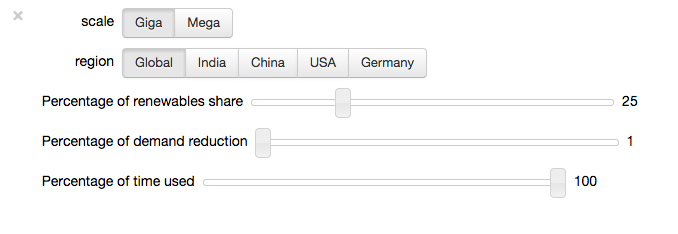
\includegraphics[scale=0.4]{interface.png}
\end{center}

\section{Conclusions}
The striking features of reviewed report are high inconsistency, lack of high-detailed methodology and model explanations, poor referencing style, and some data sources not being publicly available.\\

In the introduction, the total abatement potential is presented as $\mathbf{9.1} \mathbf{Gt}CO_2\mathbf{e}$ but simple summation of numbers presented in one of tables gives $\mathbf{9} \mathbf{Gt}CO_2\mathbf{e}$. Furthermore \emph{Manufacturing} is presented to have $\mathbf{1.2} \mathbf{Gt}CO_2\mathbf{e}$ in text and $\mathbf{1.3} \mathbf{Gt}CO_2\mathbf{e}$ in corresponding figure. Majority of errors seems to be caused by rounding and not consistent decimal accuracy. There are also different estimates of abatement potential per country appearing in the text and tables; with the worst mistake being abatement potential table for Germany being copy of US one. All these mistakes indicate poor editing and lack of sanity check before publication.\\

Furthermore, \emph{Business case assessment} figures lack indication of sources, explanation of used methodology leading to ambiguous \emph{overall business case} estimate. Major part of the report does not consider negative influence of applied ICT technology and emission of it while in use same as possible rebound effect.\\

The referencing style is not academic and is of poor quality. For large part of references it is relatively hard to find corresponding documents, and locate extracted data. Sometimes used data is outdated with newer estimates being widely available.\\

The \emph{Power} sector shows vast inconsistency in sublever naming for different countries and as mentioned above inconsistency in decimal point accuracy through \emph{the report}.\\

Majority of sublevers presented in \emph{Power} sector is highly dependant on advanced ICT-enabled smart grid infrastructure, which only can be build with strong support of the government. If building it fails majority of abatement potential in \emph{Power} sector is in danger of not being realised. Furthermore, because of high dependence, on smart-grid there is potential overlay in abatement potential which is not addressed in the report---it lacks clear boundaries between sublevers.\\

Moreover, abatement potential is highly dependant on data collection and analysis. The first one is easy to achieve but the later requires data centres and tools to extract information relevant for emission reduction.\\

Furthermore, people willingness to act upon smart meter readings and electricity price-variation is not considered in the report. Wealthy people may not care how much they pay or when they use electricity hence they lower emission abatement. It also requires some work to schedule one's task to fit into low and high tariffs which sometimes may be overwhelming.\\
For businesses consumers both these factors might be irrelevant as they may not be able to shift business operating hours to off-peak periods and businesses operating 24/7 will not benefit from it.\\

In most cases, high upfront cost of infrastructure upgrade is deterring factor. Without government subsidiaries, financing, or tax exempt it might be hard to introduce all the changes especially that majority of them has long return time.

\bibliography{le}{}
\bibliographystyle{plainnat}

\end{document}
